 \section{Relative efficiency}
\label{sec:efficiency}

 The measurement of the differential branching fraction of
 \decay{\Lb}{\Lz\mumu} relative to \decay{\Lb}{\jpsi\Lz} benefits from
 the cancellation of several potential sources of systematic
 uncertainty in the ratio of efficiencies, $\varepsilon^{\rm
   rel}=\etot(\decay{\Lb}{\Lz\mumu})/\etot(\decay{\Lb}{\jpsi\Lz})$.
 Due to the long lifetime of \Lz baryons, most of the candidates are
 reconstructed in the downstream category, with an overall efficiency
 of 0.20\,\%, while the typical efficiency is 0.05\,\% for long
 candidates.

 The efficiency of the PID is obtained from a data-driven
 method~\cite{LHCb-DP-2012-003} and found to be 98\,\% while all other
 efficiencies are evaluated using simulated data.  The models used for
 the simulation are summarised in Sec.~\ref{sec:Detector}.  The
 trigger efficiency is calculated using simulated data and increases
 from approximately 56\,\% to 86\,\% between the lowest and highest
 \qsq regions. An independent cross-check of the trigger efficiency is
 performed using a data-driven method.  This exploits the possibility
 of categorising a candidate \decay{\Lb}{\Lz\mumu} or
 \decay{\Lb}{\jpsi\Lz} decay in two ways depending on which tracks are
 directly responsible for its selection by the trigger: {``trigger on
   signal''} candidates, where the tracks responsible for the
 {hardware and software} trigger decisions are associated with the
 signal; and {``trigger independent of signal''} candidates, with a
 \Lb baryon reconstructed in either of these channels but where the
 trigger decision does not depend on any of their decay products.  As
 these two categories of event are not mutually exclusive, their
 overlap may be used to estimate the efficiency of the trigger
 selection using data.  Using \decay{\Lb}{\jpsi\Lz} candidates and
 calculating the ratio of yields that are classified as both trigger
 on signal and independent of signal, relative to those that are
 classified as trigger independent of signal, an efficiency of
 $(70\pm5)$\,\% is obtained, which is consistent with that of
 $(73.33\pm0.02)$\,\% computed from simulation.

 The relative efficiency for the ratio of branching fractions in each
 \qsq interval, calculated from the absolute efficiencies described
 above, is shown in Fig.~\ref{fig:relativeTotalEfficiency}.
 The increase in efficiency as a function of increasing \qsq is
 dominated by two effects. Firstly, at low \qsq the muons have lower
 momenta and therefore have a lower probability of satisfying the
 trigger requirements.  Secondly, at low \qsq the \Lz baryon has a
 larger fraction of the \Lb momentum and is more likely to decay
 outside of the acceptance of the detector. 
 Separate selections are used for the low- and high-\qsq regions and,
 as can be seen in Fig.~\ref{fig:relativeTotalEfficiency}, the tighter
 neural network requirement used in the low-\qsq region has
 a stronger effect on downstream candidates.
 
 The uncertainties combine both
 statistical and systematic contributions (with the latter dominating)
 and include a small correlated uncertainty due to the use of a single
 simulated sample of \decay{\Lb}{\jpsi\Lz} decays as the normalisation channel
 for all \qsq\ intervals.  Systematic uncertainties associated with the
 efficiency calculation are described in detail in Sec.~\ref{sec:systemtics}.

\begin{figure}[tbp]
%\centering \includegraphics[width=0.8\textwidth]{images_and_tables/BR/Efficiency.pdf}
\centering 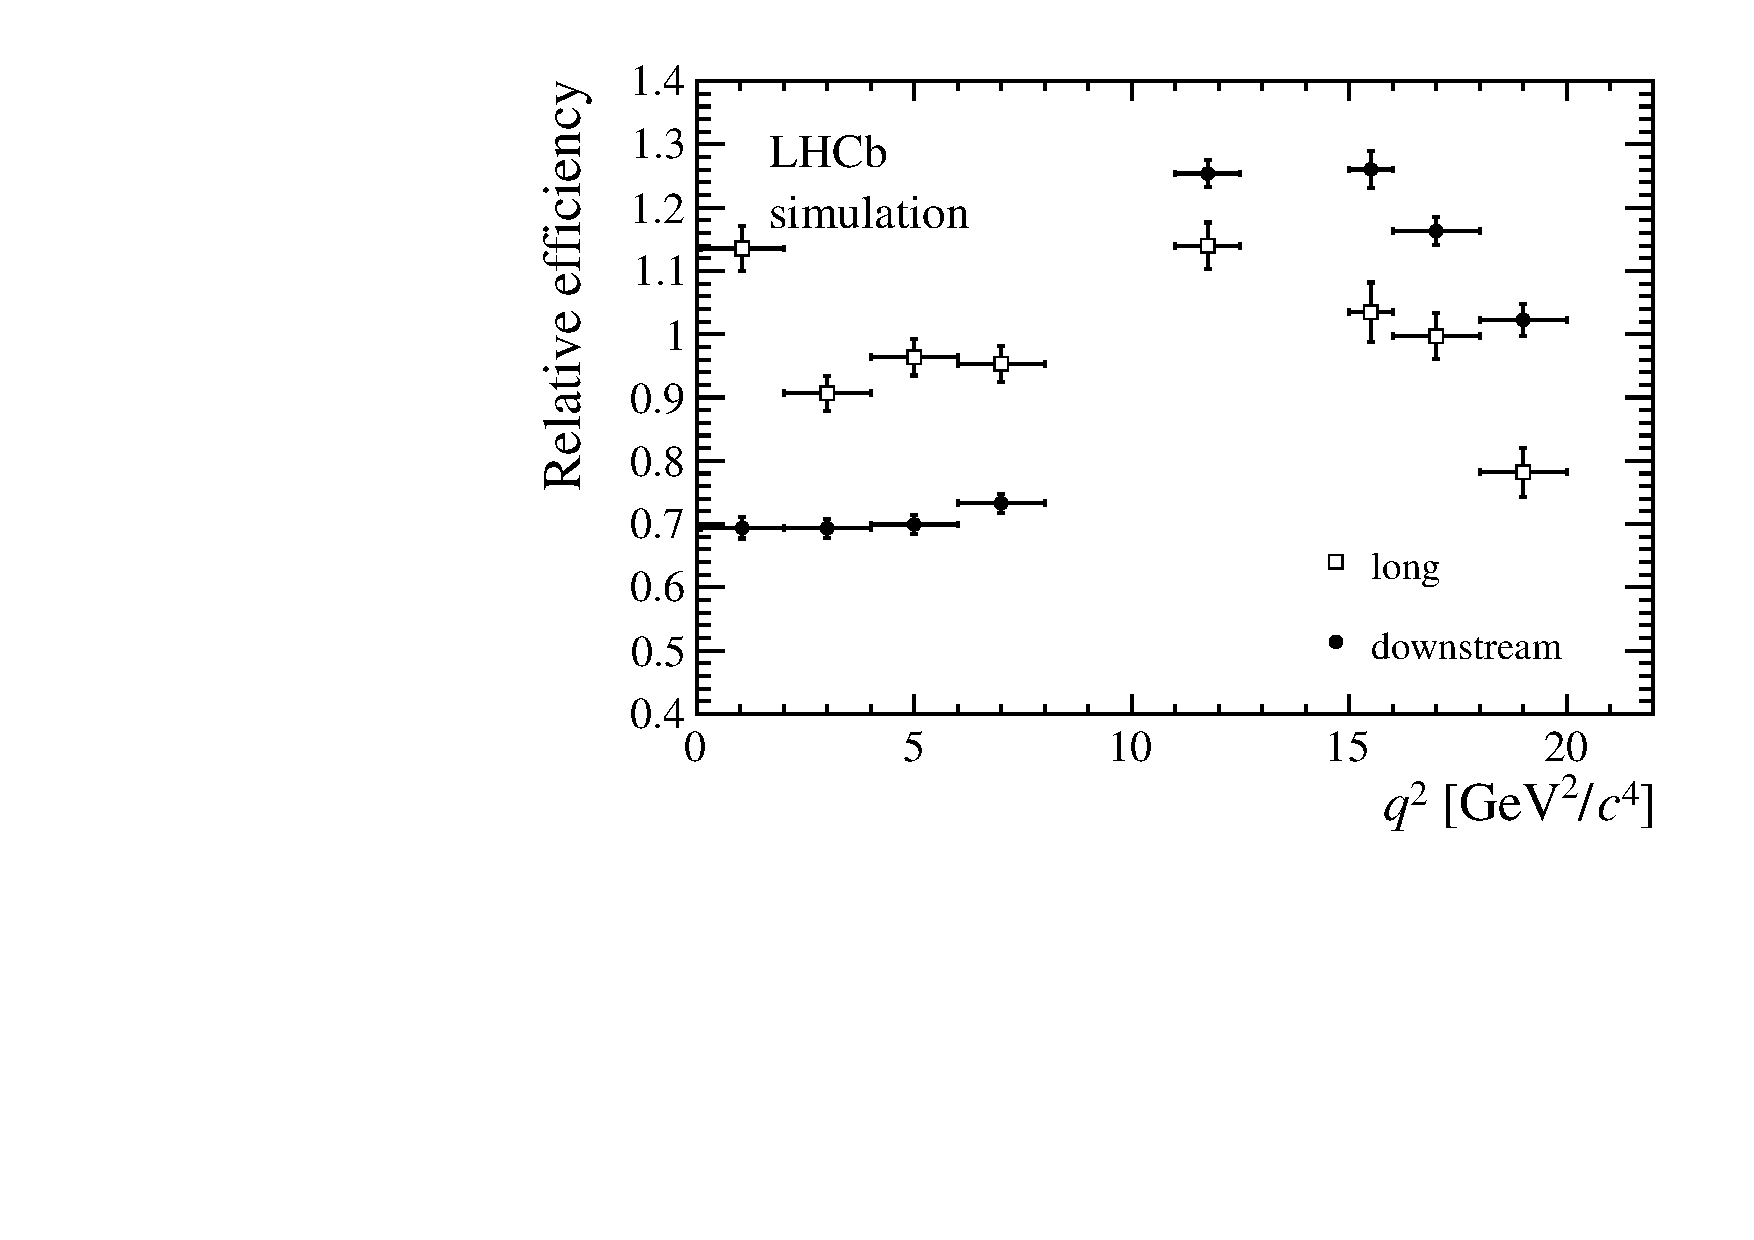
\includegraphics[width=0.8\textwidth]{figure4.pdf}
\caption{\small
Total relative efficiency,
$\varepsilon_{\mathrm{rel}}$, between \decay{\Lb}{\Lz\mumu} and
\decay{\Lb}{\jpsi\Lz} decays.
The uncertainties are the combination of
both statistical and systematic components, and are dominated by the
latter.}
\label{fig:relativeTotalEfficiency}
\end{figure}
